\begin{center}
\Huge
Kvadratkomplettering og cirklens ligning
\end{center}
\stepcounter{section}

Vi husker fra sidst, at en cirkel med centrum i $(x_0,y_0)$ og radius $r$ har ligningen
\begin{align}\label{eq:1}
	(x-x_0)^2 + (y-y_0)^2 = r^2.
\end{align}
Hæver vi parenteserne i denne ligning, så får vi
\begin{align}\label{eq:2}
	x^2+x_0^2-2xx_0 + y^2+y_0^2-2yy_0 = r^2,
\end{align}
og cirklens ligning vil ofte optræde på denne form. Kvadratkomplettering går ud på at få en ligning fra formen \eqref{eq:2} tilbage på formen \eqref{eq:1}, så radius og centrum kan aflæses.

\begin{exa}
	En cirkel har ligningen 
	\begin{align*}
		x^2-2x+y^2-4y=4.
	\end{align*}
	Vi ser, at vi har leddene $x^2$ og $-2xx_0 = -2x$ samt $y^2$ og $-2yy_0=-4y$. Derfor kan vi se, at $x_0 = 1$ og $y_0 = 2$. Ifølge \eqref{eq:2} skal vi have $x_0^2$
    og $y_0^2$ på venstresiden af lignhedstegnet, så det lægges til i cirklens ligning:
    \begin{align*}
    		x^2-2x+y^2-4y+1+4=4+1+4=9. 
    \end{align*}
   	Da ligningen nu er på formen \eqref{eq:2}, så kan vi se, at cirklen har centrum i $(1,2)$ og radius $\sqrt{9} = 3$.
\end{exa}

\section*{Opgave 1}
Bestem cirklens ligning for følgende cirkler og omskriv dem til formen \eqref{eq:2}.
\begin{center}
	\resizebox{0.45\textwidth}{0.45\textwidth}{
		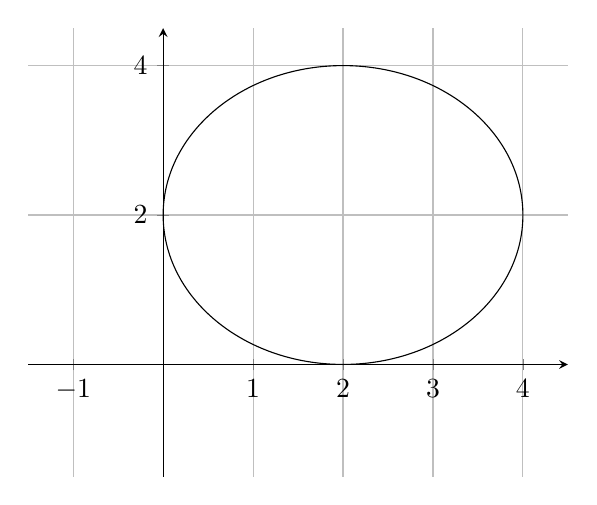
\begin{tikzpicture}
			\begin{axis}[axis lines = middle,
			xmin = -1.5, xmax = 4.5,
			ymin = -1.5, ymax = 4.5, grid]
				\draw (axis cs: 2,2) circle [blue!40, radius = 2];
			\end{axis}
		\end{tikzpicture}
	}
	\resizebox{0.45\textwidth}{0.45\textwidth}{
		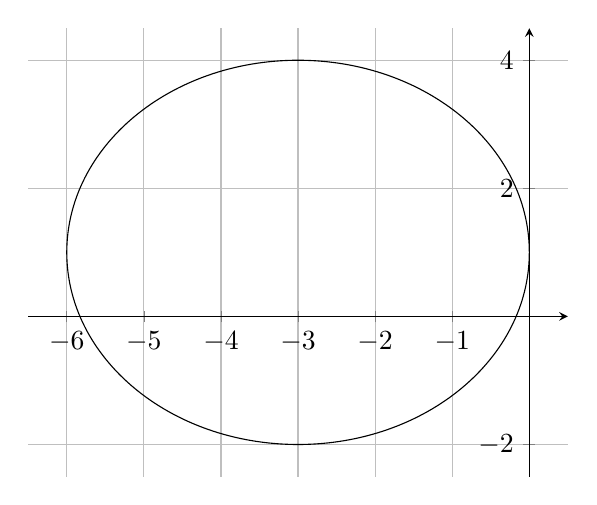
\begin{tikzpicture}
			\begin{axis}[axis lines = middle,
			xmin = -6.5, xmax = 0.5,
			ymin = -2.5, ymax = 4.5, grid]
				\draw (axis cs: -3,1) circle [blue!40, radius = 3];
			\end{axis}
		\end{tikzpicture}
	}
	\resizebox{0.45\textwidth}{0.45\textwidth}{
		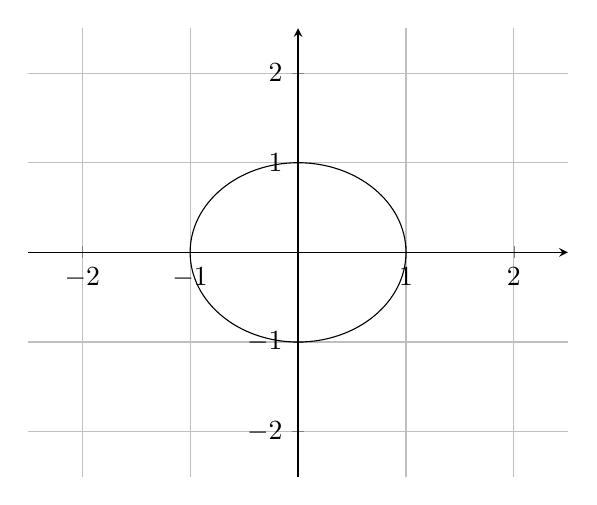
\begin{tikzpicture}
			\begin{axis}[axis lines = middle,
			xmin = -2.5, xmax = 2.5,
			ymin = -2.5, ymax = 2.5, grid]
				\draw (axis cs: 0,0) circle [blue!40, radius = 1];
			\end{axis}
		\end{tikzpicture}
	}
	\resizebox{0.45\textwidth}{0.45\textwidth}{
		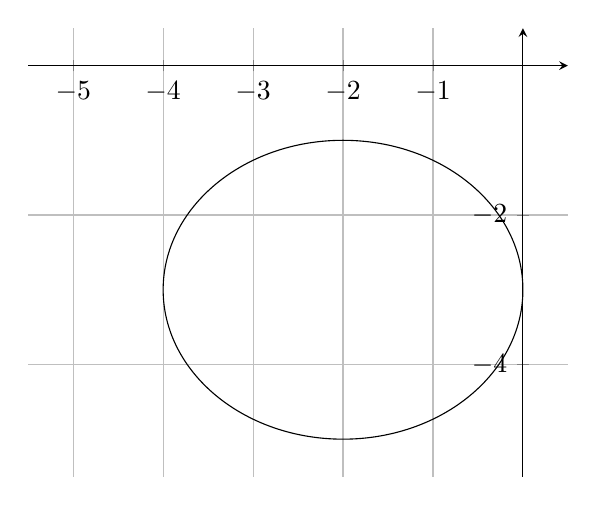
\begin{tikzpicture}
			\begin{axis}[axis lines = middle,
			xmin = -5.5, xmax = 0.5,
			ymin = -5.5, ymax = 0.5, grid]
				\draw (axis cs: -2,-3) circle [blue!40, radius = 2];
			\end{axis}
		\end{tikzpicture}
	}
\end{center}

\section*{Opgave 2}

\begin{enumerate}[label=\roman*)]
	\item Bestem centrum og radius for cirklen med ligningen
	\begin{align*}
		x^2 - 4 x + y^2 - 6 y= -9.
	\end{align*}
	\item Bestem centrum og radius for cirklen med ligningen
	\begin{align*}
		x^2 + 2 x + y^2 + 6 y = -1.
	\end{align*}
	\item Bestem centrum og radius for cirklen med ligningen
	\begin{align*}
		x^2 - 8 x + y^2 + 2 y  = 8.
	\end{align*}
	\item Bestem centrum og radius for cirklen med ligningen
	\begin{align*}
		x^2 - 10 x + y^2 - 12 y  = 3.
	\end{align*}
	\item Bestem centrum og radius for cirklen med ligningen
	\begin{align*}
		x^2 + 4 x + y^2 + 14 y = 47.
	\end{align*}
	
\end{enumerate}

\section*{Opgave 3}

\begin{enumerate}[label=\roman*)]
	\item Bestem centrum og radius for cirklen med ligningen
	\begin{align*}
		(x-4)^2+y^2-6y = 27.
	\end{align*}
	\item Bestem centrum og radius for cirklen med ligningen
	\begin{align*}
		x^2+4x+(y-3)^2 = 21.
	\end{align*}
	\item Bestem centrum og radius for cirklen med ligningen
	\begin{align*}
		x^2-14x+(y+5)^2 = 0.
	\end{align*}
\end{enumerate}
